%\section*{}
\label{sec:introduction}
\dropcap{A}s data become cheaper to gather and store, researchers have become increasingly reliant on computational workflows requiring skills in statistical modeling, machine learning and scalable computation. In addition, the recent reproducibility crises in several scientific fields has motivated the acquisition of skills in open science and the design of reproducible workflows \cite[e.g.][]{pashler2012,baker2016}.
Formal university curricula have been relatively slow to offer courses in these important topics: the slack in this area has often been picked-up by extra-curricular, ad-hoc efforts such as workshops \cite{demasi2017}.
Well-known examples are the Software and Data Carpentry workshops providing training in research computing skills through a volunteer instructor program \cite{b:wilson-swc-lessons-2016,teal2015data}.
At the same time, there has been a rise in the number of statistical and computational courses designed for specific scientific disciplines.
Examples include the \textit{Summer School in Statistics for Astronomers}\footnote{\url{http://astrostatistics.psu.edu/su16/}}, the Google Earth Engine User Summits\footnote{\url{https://events.withgoogle.com/google-earth-engine-user-summit-2017/}}, as well as a variety of project-focused (rather than pedagogical) meetings, such as the dotAstronomy meetings\footnote{\url{http://dotastronomy.com}}.
Shorter, but similar-spirit meetings have been held in conjunction with conferences, such as the Hack Days at the annual American Astronomical Society meetings, the Brainhack hackathons associated with the Organization for Human Brain Mapping and the Society for Neuroscience\cite{Cameron_Craddock2016-wc}, and a hackathon at the American Geophysical Union meeting\footnote{\url{http://onlinelibrary.wiley.com/doi/10.1002/2014EO480004/pdf}}. 
In general, many of these events tend to emphasize either a more traditional pedagogical class and lecture methodology, or emphasize a focus on ad-hoc projects that participants work on during the event (Figure \ref{fig:hackspectrum}).
Pedagogically-focused events follow a classic academic model where novices learn new skills from experts. This model tends to focus on a one-way flow of information from instructor to student, and are usually targeted towards participants in the training phase of their career. On the other end of the spectrum, project-focused workshops emphasize collaborative activities using existing skills, leading to the common perception that they are designed for technical experts, and this may limit their audience. 
To bridge this gap, we describe here a model that we have implemented: ``Hack Weeks'' that aim to capitalize on the advantages of each of these models.
These week-long events combine structured periods focused on pedagogy (often with an emphasis on statistical and computational techniques) with less structured periods devoted to hacks and creative projects, with the goal of encouraging collaboration and learning among people at various stages of their career. 

%Our hack week model shares some similarities to those summer schools that combine individual or group project work with teaching methods that transfer knowledge from experts to early-career researchers.
%However, a distinguishing factor of our hack weeks in that they tend to be less structured and more participant-driven, so that the learning content is co-created between organizers and participants based on the unique experience of people in the room. 

\begin{figure}
\begin{center}
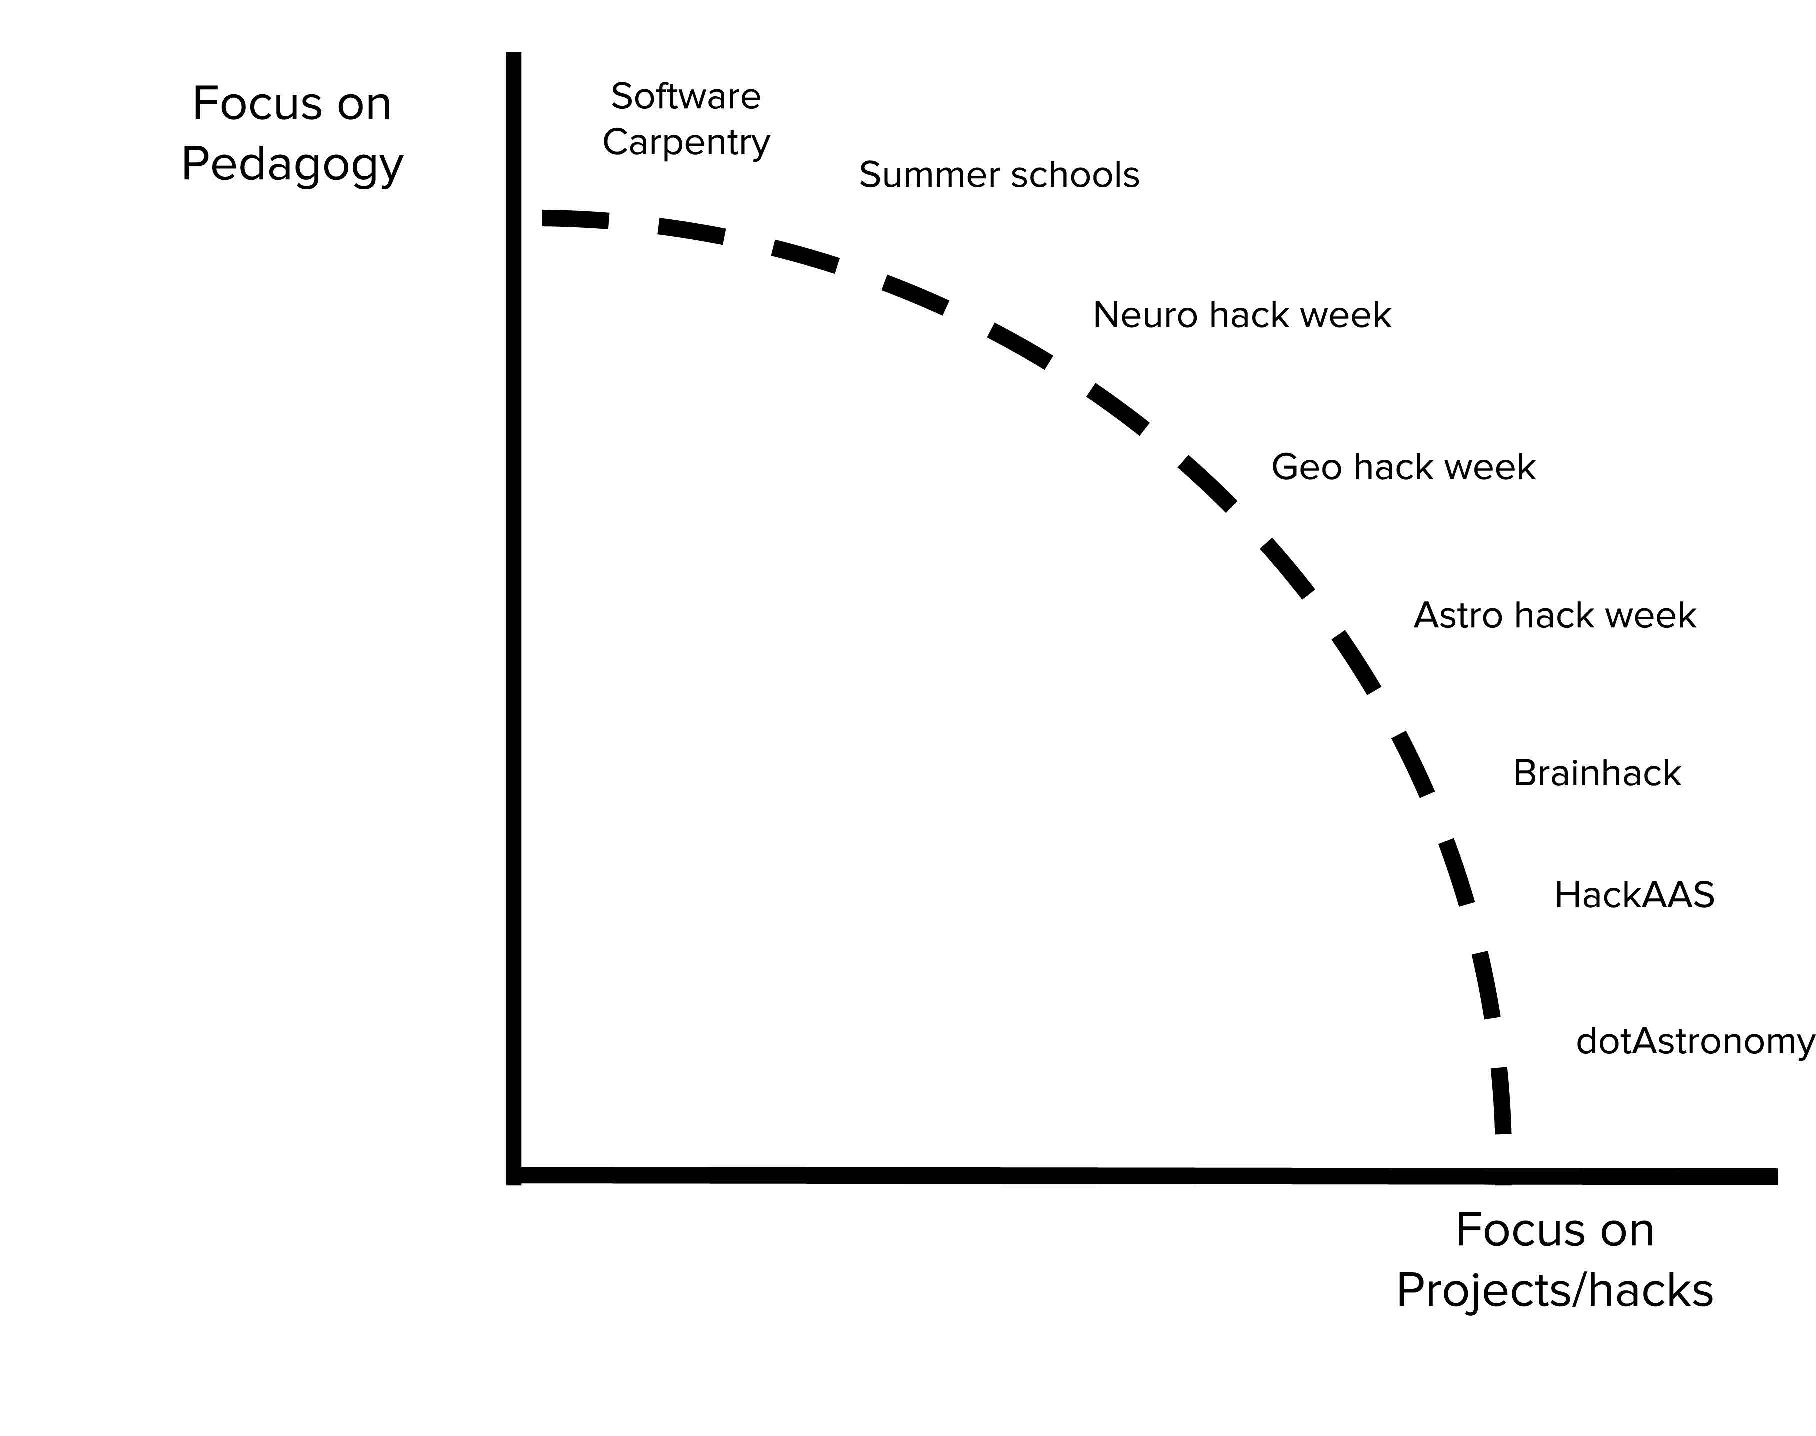
\includegraphics[width=8cm]{NewHackSpectrum.pdf}
\caption{{\bf Comparison of Extracurricular Workshop Models}: Different types of events lie on a spectrum between the emphasis on pedagogy (e.g. Software Carpentry workshop) to an emphasis on project-based/hack-based activities (e.g. at science-oriented hackathons). Hack weeks also vary in the degree of emphasis on projects (e.g. Astro Hack Week) or pedagogy (e.g. Neuro Hack Week)}
\label{fig:hackspectrum}
\end{center}
\end{figure}

As of the publication of this paper, we have run eight such hack week events: four focused on Astronomy, and two each focused on Neuroscience and Geoscience.
Here we share the philosophy behind the hack week model, results from surveys of participants, practical lessons we have learned in organizing these events, and recommendations for future hack weeks. Supplementary materials (SM) provide additional details on the practical aspects of organizing these events.
